%
% Humanoids 2006 submission
% Optimising SVMs for robotic control
% Castellini, Orabona, Sandini
%

\documentclass[conference]{IEEEtran}
\usepackage{amsmath}
\usepackage[psamsfonts]{amssymb}
\usepackage{amsbsy}
\usepackage{url}
\usepackage{graphicx}

\def\RR{\mathbb{R}}
\def\NN{\mathbb{N}}
\def\xx{\mathbf{x}}
\def\ww{\mathbf{w}}
\def\aa{\boldsymbol{\alpha}}
\def\bb{\boldsymbol{\beta}}
\def\ee{\mathbf{e}}
\def\dd{\mathbf{d}}
\def\mdd{\tilde{\dd}}
\def\b{\mathcal{B}}
\def\d{\mathcal{D}}

\begin{document}

\title{Optimised Support Vector Machines\\for Robotic Control}
\author{
\authorblockN{Claudio Castellini and Francesco Orabona and Giulio Sandini}
\authorblockA{LIRA-Lab, University of Genova\\
viale F. Causa, 13 - 16145 Genova, Italy\\
email: claudio.castellini@unige.it}}

\maketitle

\pagestyle{empty}
\thispagestyle{empty}

\begin{abstract}

  Support Vector Machines (SVMs) are a machine learning method rooted
  in statistical learning theory, able to classify data and perform
  regression on it. Their main advantages with respect to other
  similar methods such as, e.g., artificial neural networks, are that
  $(a)$ they rely upon a solid theoretical background, $(b)$ they are
  stable, their training always ending up in a global minimum of the
  objective function, and $(c)$ they easily generalise to
  high-dimensional feature spaces.

  Surprisingly, they have so far been little used in robotic control,
  possibly due to their supposed inability to cope with very large
  datasets; in this paper we apply SVMs to robotic control, namely to
  the problem of finding direct and inverse models of arm/head/eye
  systems, and introduce three optimisations which, on the chosen
  problems, effectively reduce the size of the required datasets,
  while retaining most of the accuracy.

  The result is a learning method which can be applied online, since
  the time required to train the associated machine is much shorter
  than without the proposed optimisations.

\end{abstract}

\section{Introduction}

Introduced by Boser, Guyon and Vapnik in the early 90s \cite{BGV92},
Support Vector Machines (SVMs) are a class of machine learning
algorithms characterised by the use of kernels, the absence of local
minima, the sparseness of the solution and the ability to control the
machine capacity by maximising quantities which are independent of the
dimension of the input space. So far, they have been successfully
used, e.g., in text categorisation, image recognition, hand-writing
recognition and bioinformatics \cite{Cristianini00}. Their good
theoretical properties make them suitable both for classification
(guessing the category of a datum) and regression tasks (approximating
an unknown function).

Possibly due to their alleged inability to cope with large datasets,
so far they have not been used extensively in robotic
control. Especially, this has ruled out building on-line SVM-based
kinematic models; a typical example would be that of a supervised
training phase in which a robot samples its joint space while
gathering perceptual data about the position of its limbs in the
Cartesian space. Such a learning system should indeed do regression on
its own body's model, being then able, in the test phase, to reach for
any point in its workspace by generalising the examples seen in the
training phase.

But indeed, one of the most interesting characteristics of SVMs is the
\emph{sparseness} of the solution, meaning that a few samples account
for the whole complexity of the problem. In other words, it is a
matter of detecting what the robot should do during the training phase
in order to achieve a good accuracy in the approximation of its
kinematic inverse model. This would also pave the way for
\emph{online} SVM-based learning of a kinematic model, since a smaller
machine can be trained in a cubically shorter time
\cite{KeerthiCDC06}, making it feasible to train \emph{while}
gathering data \emph{and} controlling the robot limbs.

In this paper we try to fill this gap by proposing three optimisations
to SVMs which actually reduce their size, while retaining most of the
accuracy of the full machines. Our experimental results show that, at
least in two cases, our optimisations lead to good results, namely:
$(a)$ building a direct kinematic model of a teleoperation master
setup composed of a magnetic tracker and a pair of cameras, $(b)$
building an inverse kinematic model of the arm/head/eyes system of a
humanoid robot. Although we haven't yet built real on-line versions of
our optimisations, this eases future research in this topic.

The paper is structured as follows: in Section \ref{sec:bg} we
introduce some background notions proper to robotic kinematic models
and SVMs; in Section \ref{sec:opt} we describe our optimisations; in
Section \ref{sec:exp} we show the experimental results, and lastly in
Section \ref{sec:concl} conclusions are drawn, and future work is
outlined.

\section{Background}
\label{sec:bg}

\subsection{Kinematic models}
\label{subs:kinmod}

Consider the problem of building a kinematic model of a robotic
system composed of a multi-DOF arm and head, and a stereo vision
system, usually two cameras mounted on the head. The problem we are
interested in is that of mapping the proprioceptive data coming from
the head and arm (i.e., the positions of the head and arm joints) to
the perceptual data seen by the robot eyes. Essentially, we want the
robot to associate the position of its limbs to their images, as
perceived by the cameras --- a task which bears some resemblance to
what human infants learn in their early stages of life (see, e.g.,
\cite{VonHofsten2004}). This problem will be referred to as
\emph{direct} kinematic problem, whereas the \emph{inverse} problem
will be that of deducing from vision what to command to the limbs in
order to reach for a point in the robot workspace. Notice that this is
a similar problem to the standard formulation of the inverse
kinematics problem, in which a map from the Cartesian space to the
joints space is sought for.

The problem is quite hard if na\"\i vely tackled, since, e.g., the
number of degrees of freedom can be higher than the dimension of the
output space, leading to redundancy. Additionally, it is at this stage
unclear what features of robotic vision we should be monitoring; using
raw data coming from the cameras seems impracticable, since the system
should have some \emph{a priori} notion of what it should be tracking.

We then concentrate on two simpler problems: first, the direct
kinematic model of a teleoperation master setup; second, the inverse
kinematic model of a humanoid arm/head/hand system.

In the first problem, a master teleoperation setup is available,
mainly composed of two fixed stereo cameras and an Ascension
\emph{Flock of Birds} magnetic tracker (see Figure
\ref{fig:setup}, plate $(a)$). The tracker sensor is attached on the user's wrist
and a red marker is applied on it; light and colour conditions are
carefully controlled in order for the sensor to be easily segmented in
the camera images. The tracker records real-time the Cartesian
position of the sensor. So we want to build a map between the sensor
position in 3D space and its position in the camera spaces.

In the second problem, we have gathered a data set from the Babybot
humanoid setup \cite{babybotHum2005}. The setup consists of a 6DOFs
PUMA robotic arm, a custom built 6DOFs humanoid hand, a 5DOFs robotic
head and two cameras (see Figure \ref{fig:setup}, plate $(b)$). The
data set consists of the positions of three joints of the arm
(shoulder, elbow and wrist) and the three component of the vector
$\mathbf{v} = (v_x,v_y,v_z)$, representing the position of the hand in
the head-centered reference frame (i.e., with respect to the base of
the head/neck). The vector $\mathbf{v}$, together with the angles of
the head joints, uniquely determines the position of the hand in the
image plane (for more details, see \cite{NatalePhD}). The aim here is
to build a map between proprioceptive data coming from the arm and the
position of the hand \emph{as seen by the robot} (see Figure
\ref{fig:setup}, plate $(c)$).

\begin{figure*}[!htbp]
  \begin{center}
    \begin{tabular}{ccc}
      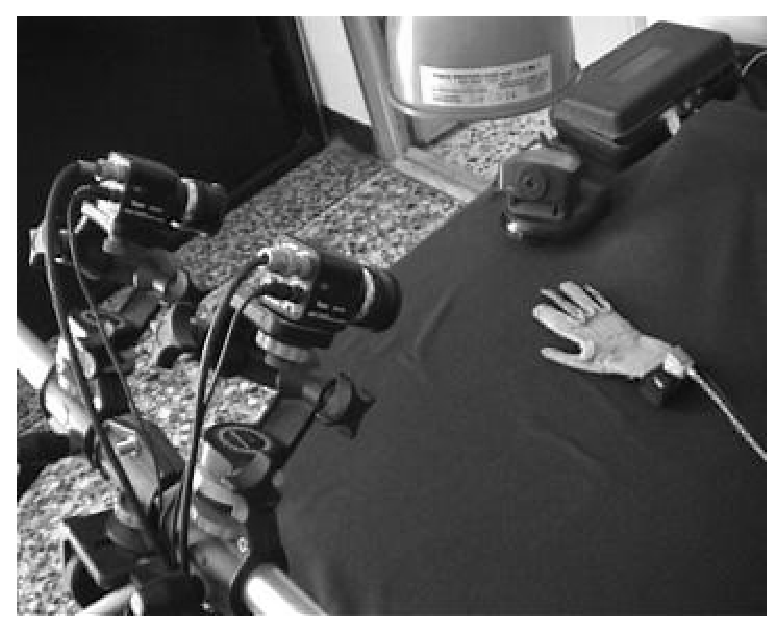
\includegraphics[width=0.31\textwidth]{master} &
       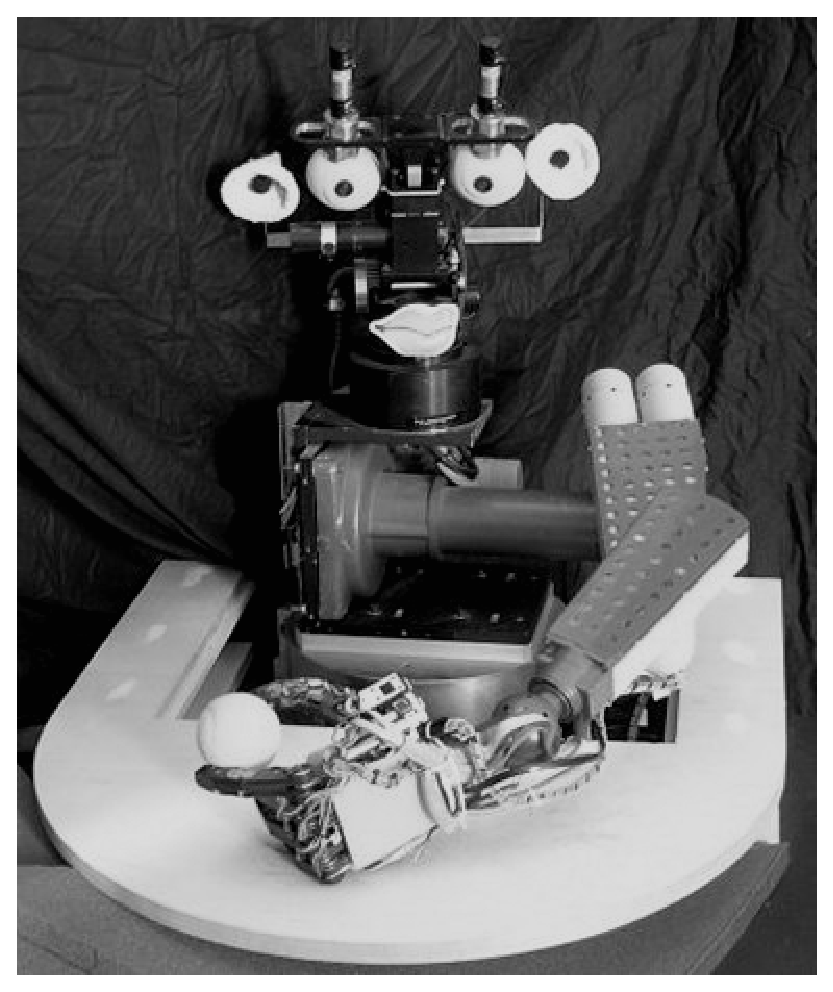
\includegraphics[width=0.31\textwidth]{babybot} &
       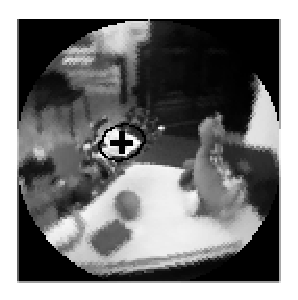
\includegraphics[width=0.31\textwidth]{pov} \\[5mm]
       (a) & (b) & (c)
    \end{tabular}
  \end{center}
  \caption{\label{fig:setup} Experimental setup. $(a)$ the master
  teleoperation setup, including the cameras and the Flock-Of-Birds
  magnetic tracker, attached on the wrist of a data glove; $(b)$ the
  Babybot humanoid setup; $(c)$ what Babybot sees when it locates its
  own hand.}
\end{figure*}

\subsection{Support Vector Machines}
\label{subs:svm}

Due to space limitations, and since this material is totally standard,
this is a very quick account of SVMs --- the interested reader is
referred to \cite{Burges98,SmolaTut2004} for a tutorial, and to
\cite{Cristianini00} for a comprehensive introduction to the subject.

\subsubsection{Linear classification of separable data}

Assume $\{\xx_i,y_i\}_{i=1}^l$, with $\xx_i \in \RR^m$ and $y_i \in
\{-1,1\}$, is a set of \emph{samples} drawn from an unknown
probability distribution; each sample is a point in the \emph{input
space} $\RR^m$ and a \emph{label}, so that the points are classified
in two ``groups''. The aim is that of approximating the distribution
in order to predict more data coming from the same source to the best
extent possible. Let us assume for now that the two groups are
\emph{linearly separable}, meaning that there exists a linear function
in $\RR^m$ (hyperplane) such that each group lies entirely on one side
of the hyperplane. There are in general infinite such hyperplanes; we
wish to find the one which maximises its own distance from both groups
of samples (\emph{margin}).

Such a hyperplane looks like $\ww\cdot\xx + b$, where $\ww \in \RR^m$
and $b \in \RR$, and it is easy to check that the margin is
$\frac{2}{||\ww||}$. In order for the samples to be correctly
classified, it must hold that $y_i(\ww\cdot\xx_i + b)-1\geq 0$, for
all $i=1,\ldots,l$. Such a problem can then be compactly expressed in
Lagrangian form, by introducing $l$ coefficients $\alpha_i$ and then
trying to minimise the objective function

$$ L(\ww,b,\aa) = \frac{1}{2}||\ww||^2 -
                  \sum_{i=1}^{l} \alpha_i y_i(\ww\cdot\xx_i + b) +
                  \sum_{i=1}^{l} \alpha_i $$

\noindent subject to the constraints that $\alpha_i\geq 0$ for all
$i$s. For reasons that will be clearer later on, rather than
minimising $L(\ww,b,\aa)$, it is standard to maximise its \emph{dual}
form, obtained by applying the extremum conditions $\nabla_{\ww,b}
L(\ww,b,\aa) = 0$:

$$ L_D(\aa) = -\frac{1}{2} \aa^T D \aa + e^T \aa $$

\noindent where $\ee$ is the vector of $l$ ones,
$D_{ij}=y_iy_j\xx_i\cdot\xx_j$, and subject to $\sum_{i=1}^{l}
y_i\alpha_i = 0$ and $\aa \geq 0$ (meaning that all components of
$\aa$ must be greater than or equal to zero). Once a minimum for
$L_D(\aa)$ has been found, the resulting $\aa$ can be easily used to
recover $\ww$ and $b$ and therefore the decision function. In
particular, the expression for $\ww$, directly derived from the
extremum condition, is

$$ \ww = \sum_{i=1}^{l} \alpha_i y_i \xx_i $$

\noindent in which it is apparent that, in building the decision
function, the Lagrange coefficients introduced in the minimisation
problem appear as \emph{weights} of the training data. It is
well-known that some of the $\alpha_i$s (actually most of them in many
practical applications) are zero; those $\xx_i$s for which this does
\emph{not} hold are crucial to the solution and are called
\emph{support vectors}, hence the name of the approach. This
phenomenon is known as \emph{sparseness} of the solution, meaning that
only a subset of the training data is usually really needed to build
it.

Notice, moreover, that both formulations are convex quadratic
programming problems, therefore gifted with a (possibly non-unique)
global solution. A smart minimisation algorithm will therefore always
find the right solution at the first attempt, without risking being
trapped in local minima, as is the case, e.g., with artificial neural
networks.

\subsubsection{Extensions}

The above sketched approach can be easily extended at least in three
orthogonal directions.

\begin{enumerate}

  \item Lifting the assumption that the data are indeed separable, the
    very same machinery can be applied, at the price of introducing
    $l$ \emph{slack variables} $\xi_i$ which control how hard each
    constraint is. The resulting dual cost function is still
    $L_D(\aa)$ but now subject to $\sum_{i=1}^{l} y_i\alpha_i = 0$ and
    $0 \leq \aa \leq C$, where $C \in \RR$ can be used to trade more
    classification errors versus a larger margin.

  \item If a suitable set of features of the input space can be found,
    then a non-linear mapping $\Phi(\xx)$ can be applied to project
    the data in a highly dimensional \emph{feature space}. The
    explicit mapping $\Phi(\cdot)$ need not be known --- in fact, all
    is needed is a function
    $K(\xx_1,\xx_2)=\Phi(\xx_2)\cdot\Phi(\xx_2)$ (often called
    \emph{kernel}) evaluating dot products in the feature space. Since
    the $\xx_i$'s only appear as dot products in $D$, one only needs
    replacing them with the corresponding element of the \emph{kernel
    matrix} $K$, where $K_{ij} = K(\xx_i,\xx_j)$.

  \item \emph{Regression} (approximating an unknown function, rather
    than classifying data) can be efficiently done along the same
    lines, at the price of introducing a threshold $\epsilon>0$
    stating how close we want the approximate function to be to the
    target function.

\end{enumerate}

Putting together cases $2$ and $3$ above, one can view SVMs for
regression as function approximators which linearly combine elements
from a Hilbert space to build a model of the target function. The
space, and therefore the building blocks of our approximation, depend
on the choice of the kernel. Several standard kernels have been
defined and employed. In this paper we will focus on one of the most
common choices, that of Gaussian kernels; the choice is also motivated
by the fact that, under some conditions, these kernels subsume the
linear ones \cite{KLAsympt}. As a result, our machines will
approximate the target function by means of a function

$$ f(\xx) = \sum_{i} \alpha_i e^{-\frac{||\xx-\xx_i||^2}{\sigma^2}} $$

\noindent for a fixed $\sigma$.

\subsubsection{Implementation}

A number of algorithms for minimising the cost function associated to
a SVM, either in its primal or dual form, have been proposed. Willing
to focus upon the practical, on-line use of SVMs on a robot, we have
decided to use an off-the-shelf SVM package, which could be both used
within MatLab for fast prototyping and then encapsulated in a C++
environment, to be shipped aboard robots. We have therefore chosen
\emph{LIBSVM} v2.81 \cite{ChangL01}.

\section{Support Vector Machines for Robotic Control}
\label{sec:opt}

In this Section we describe our optimisations to SVM regression for
robotic control. As said in Section \ref{sec:bg}, one of the most
interesting advantages of SVMs is the sparseness of their solution; it
seems therefore reasonable to try and look for (possibly heuristic)
strategies to avoid acquiring samples which will then be neglected in
the solution, or to filter out useless samples from the sample
pool. This is the main idea behind the strategies we describe below.

\subsection{Uniform Sampling (US)}

For the problems described in Subsection \ref{subs:kinmod}, it is
reasonable to assume a certain continuity in the map we are after ---
both problems are about mapping a continuous space to another
continuous one. Consider, e.g., the second problem: neglecting
pathological cases, nearby positions of the robotic hand will result
in ``nearby'' positions in the joint space, and vice-versa. This
suggests that samples which are too close to one another in the input
space can be useless.

Assume for instance that the input space is $\RR^m$, and that a set of
$l$ samples, as described in Subsection \ref{subs:svm}, is available
(this is the case of the first problem considered, see Subsection
\ref{subs:kinmod}); also, let $\theta \in \RR$ be a threshold
parameter. Then when a new sample $\xx_{l+1}$ is gathered, follow this
rule:

\begin{itemize}
  \item if $||\xx_{l+1}-\xx_i|| > \theta$ then add $\xx_{l+1}$ to
    the current sample set; otherwise, ignore it.
\end{itemize}

\noindent (In more complex cases a separate threshold should be set
for each dimension of the input space.) Especially in an online
environment, where new training samples are gathered as the movement
of the setup goes on, this strategy prevents samples which are too
close to one another to be stored in the training set. For example, in
the first problem, in which the input space is the 3D Cartesian space,
setting the threshold will force the system to sample the space
uniformly at one sample per each sphere of radius $\frac{\theta}{2}$.

\subsection{Error-Based Sampling (EBS)}

Assume, again, $l$ samples have been gathered so far and the SVM has
been trained on them. It seems reasonable, then, to avoid sampling the
input space where the prediction of the SVM is already accurate
enough. Let $f(\xx)$ be the target function approximation built so far
using the SVM, as described in Subsection \ref{subs:svm}, and let
$\delta \in \RR$ be a threshold constant. Then when a new sample
$\xx_{l+1}$ is gathered, follow this rule:

\begin{itemize}
  \item if $|f(\xx_{l+1})| > \delta$ then add $\xx_{l+1}$ to the
    current sample set; otherwise, ignore it.
\end{itemize}

This can be seen as a sort of feedback control over the sampling
procedure: if the current model is ``not that wrong'' about the
candidate sample, we do not consider it. Again, this is especially
useful in an online environment, since, by the hypothesis of
continuity of the maps stated in the previous Subsection, the farther
we get from a point which the model already predicts well, the worse
the prediction will be (assuming we are moving to a zone of the input
space which hasn't been sampled yet).

We have found it convenient to set this threshold at a multiple of the
regression threshold $\epsilon$ (see Subsection
\ref{subs:svm}). Notice that setting it at $\epsilon$ makes the system
precise, in the sense that if the model's prediction at some point is
already within $\epsilon$, the current solution is optimal.

\subsection{Non-SV Filtering (nSVF)}

In \cite{syed99incremental}, where the problem of
\emph{classification} rather than that of regression is tackled, the
idea is proposed that in an online environment, if we neglect
completely the samples which are not support vectors, the result
should not change too much. In that paper experimental results are
shown which corroborate the thesis, and also show that if we remove
even a small fraction of the support vectors, the accuracy of the
system drops dramatically. The reason behind this is the sparseness of
the SVM solution: essentially, all the information needed to build the
decision surface is contained in the support vectors, which are
usually a small fraction of the training samples.

According to this idea, whenever training is performed, we follow this
rule:

\begin{itemize}
  \item for each $i=1,\ldots,l$ if $\xx_i$ is not in the set support
    vectors, then erase it.
\end{itemize}

\section{Experimental Results}
\label{sec:exp}

In order to check the effectiveness of the above presented strategies,
we have tested them on the two problems detailed in Subsection
\ref{subs:kinmod}. We compare a ``plain'' implementation of LIBSVM
with the three strategies, US, EBS and nSVF; EBS comes in two
variants, one in which $\delta = 10\epsilon$ and one in which $\delta
= 50\epsilon$. For the sake of qualitative comparison, later on, we
also show results coming from Schaal's Receptive Fields Weighted
Regression (RFWR, \cite{schaal98constructive}), a bio-inspired machine
learning system in which function approximation is achieved
incrementally by locally training single learning units. It must be
remarked that RFWR is completely on-line, that is, the system retains
no knowledge of the past samples but only trains the network according
to the new sample; whereas at this stage our system works in batch
mode: training is performed after $n$ samples have been acquired. The
parameter $n$ has been, so far, arbitrarily set to $10$. RFWR is,
moreover, a piece of MatLab code, therefore we do not compare CPU
times.

For each problem, we have first performed a comparison among various
combinations of the three strategies. Clearly, US and EBS are
competitive to each other; therefore we have considered, besides the
three strategies on their own, the combinations nSVF+US and nSVF+EBS,
with both settings of EBS. The assumption, which we have
experimentally verified, is that there is a tradeoff between accuracy
and compactness. Among all the strategy combinations, we have chosen:
$(a)$, that which achieves the smallest machine, that is, which
reduces most the number of samples; $(b)$, that which achieves the
best performance error, thus retaining the best accuracy; and lastly
$(c)$, that with the best tradeoff, that is, with a reasonably low
error but also with a good reduction factor.

For each of the two problems we present two graphs: the left-hand
panels show the reduction of the machine size achieved by each
strategy (or combination of strategies) as a percentage of the size of
the plain SVM; whereas the right-hand panels compare the absolute
sizes of the strategy with the best trade-off found in the left-hand
graph, of the plain SVM, and of Schaal's RFWR. The \emph{size} is
defined as the number of support vectors for the SVMs, and the number
of receptive fields for the RFWR. This seems reasonable, since
receptive fields are added by the RFWR strategy ``as they become
necessary'' to the approximation.

\subsection{Direct model of a teleoperation master setup}

Figure \ref{fig:teleop} shows the results for the teleoperation
setup.

\begin{figure*}[!htbp]
  \begin{center}
    \begin{tabular}{cc}
       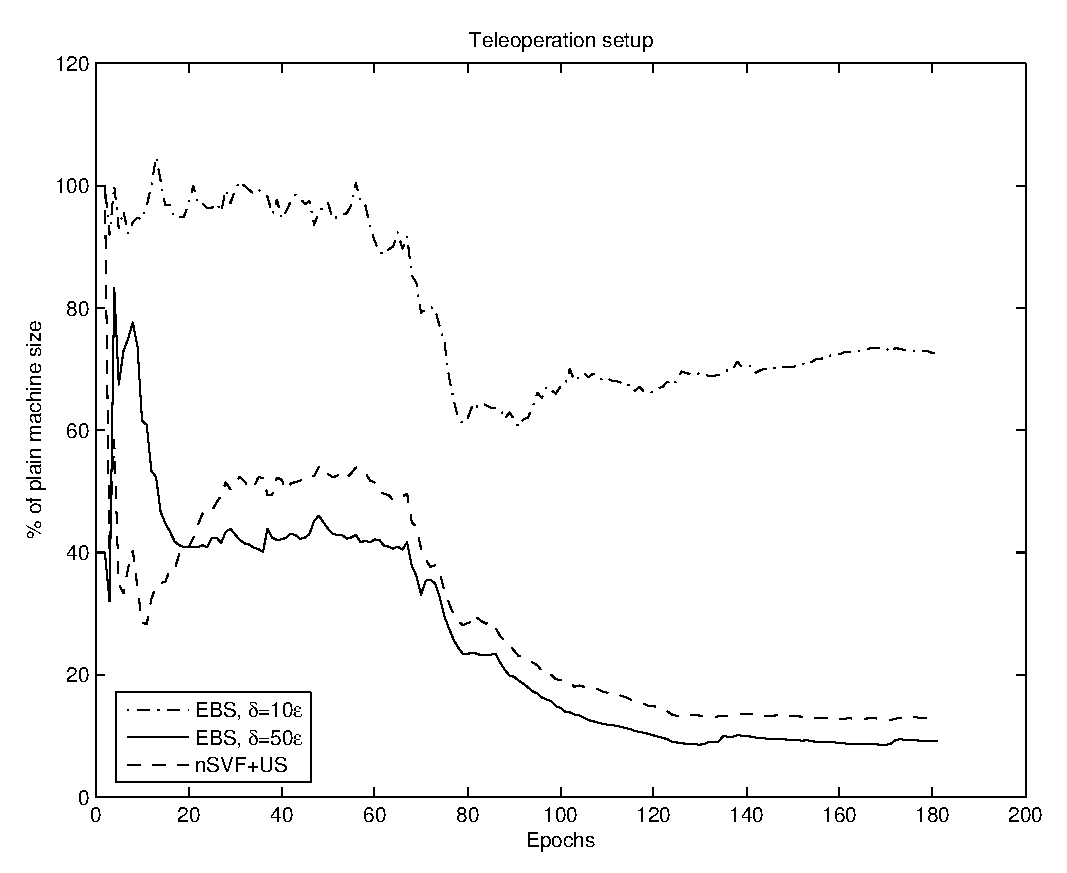
\includegraphics[width=0.45\textwidth]{fig3b} &
       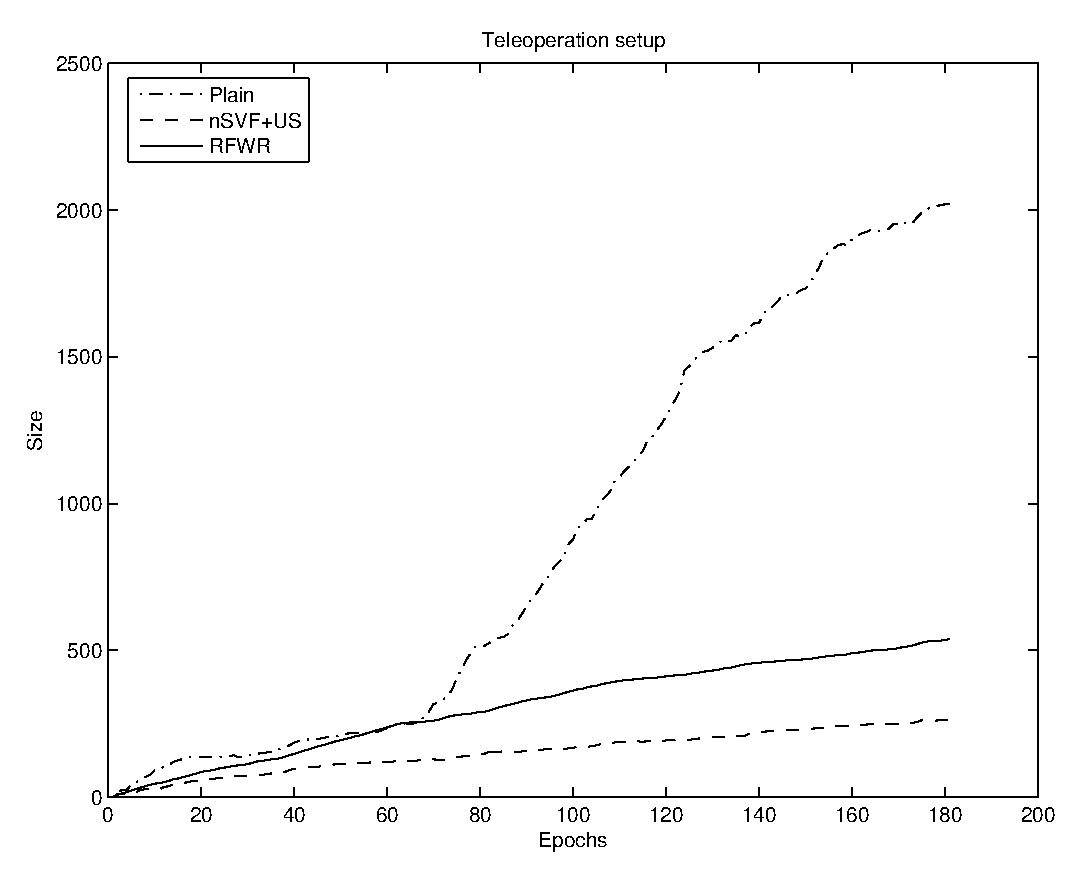
\includegraphics[width=0.45\textwidth]{fig4b} \\[5mm]
       \multicolumn{2}{c}{
         \begin{tabular}{|l|r|r|}
           \hline
           Machine & Size & MSE \\
           \hline\hline
           Plain                    & $100\%$   & $0.0087$ \\
           EBS, $\delta=10\epsilon$ &  $72.7\%$ & $0.0092$ \\
           EBS, $\delta=50\epsilon$ &   $9.2\%$ & $0.0234$ \\
           \bf nSVF+US              &  $13.1\%$ & $0.0165$ \\
           RFWR                     &       - & $0.0275$ \\
           \hline
         \end{tabular}
       }
    \end{tabular}
  \end{center}
  \caption{\label{fig:teleop} Experimental results for the
    tracker-to-eyes teleoperation setup mapping (see Subsection
    \ref{subs:kinmod}). \emph{Above left:} percentage of the plain
    machine size, as a function of the epochs. Comparison among EBS
    with $\delta=10\epsilon$, EBS with $\delta=50\epsilon$ and
    nSVF+US. \emph{Above right:} The strategy with the best trade-off
    as resulting from the left panel, i.e., nSVF+US, compared with the
    plain SVM and Schaal's RFWR. \emph{Below:} numerical data: for
    each plotted machine, final size as a percentage of the plain SVM
    and MSE of the regressions obtained. The strategy with the best
    tradeoff appears in boldface.}
\end{figure*}

First of all, consider the numerical table below the graphs: as
expected, it is apparent that there is a trade-off between accuracy
and size: the smaller the machine, the worse the Mean Square Error
(MSE) of the approximation achieved at the end of the training. Notice
that the strategy with the best trade-off, i.e., nSVF+US, obtains a
machine which is $13.1\%$ of the plain machine at the price of
doubling the MSE.

Consider now the above left graph: notice that the curves somehow
settle to a constant value after some epochs, indicating that the
growth is actually being contained. (Also, notice that one of the
optimisations, for a brief time, outsizes the plain SVM.) For
instance, the EBS with $\delta=50\epsilon$ strategy generates a
machine which remains, in the long run, about one-tenth of the size of
the plain SVM. One has to remember that this does \emph{not} mean that
the machines stop growing, but rather that they \emph{constantly grow
less}. In agreement with a recent result by Steinwart
\cite{Steinwart03}, their growth is linear with the number of acquired
samples, but it is a flatter linear function.

Consider now the above right graph. The size of the machine employing
the strategy nSVF+US remains about half the size of the RFWR, while
achieving an error which is about $0.6$ times that of RFWR.

\subsection{Inverse model of a humanoid arm/head/eyes setup}

Figure \ref{fig:hum} shows the results for the humanoid setup.

\begin{figure*}[!htbp]
  \begin{center}
    \begin{tabular}{cc}
       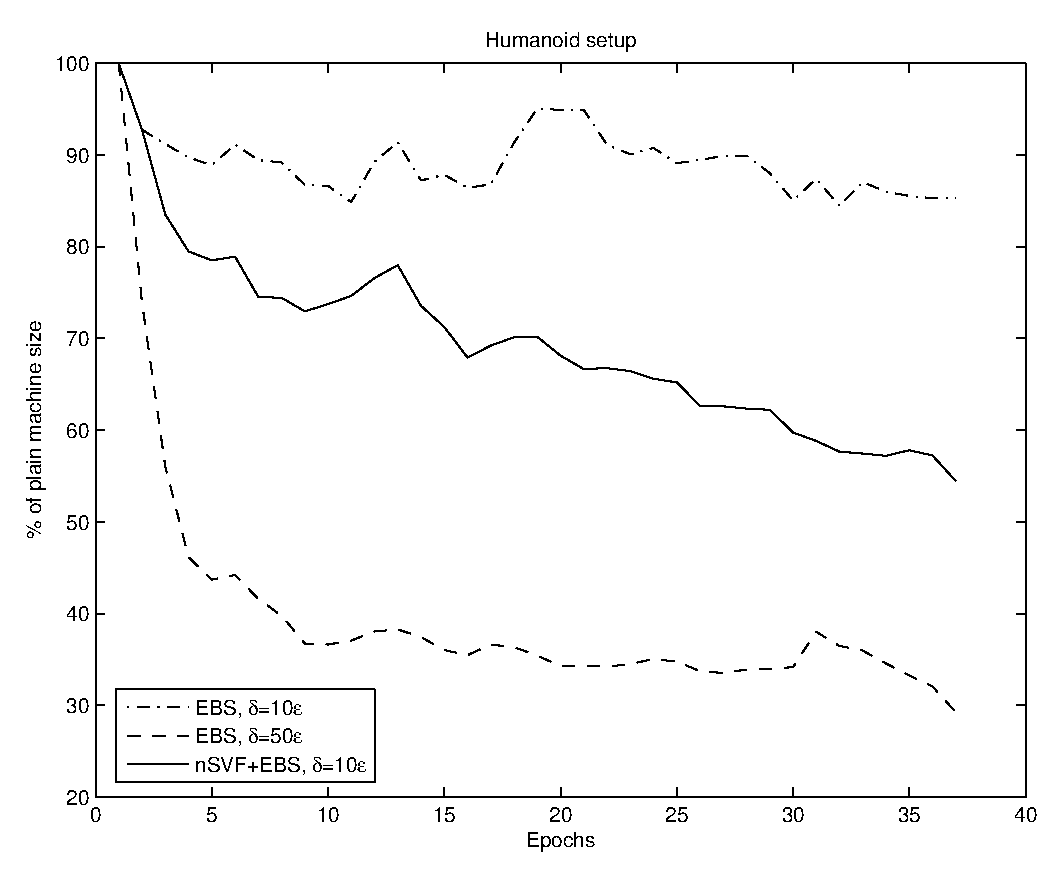
\includegraphics[width=0.45\textwidth]{fig1b} &
       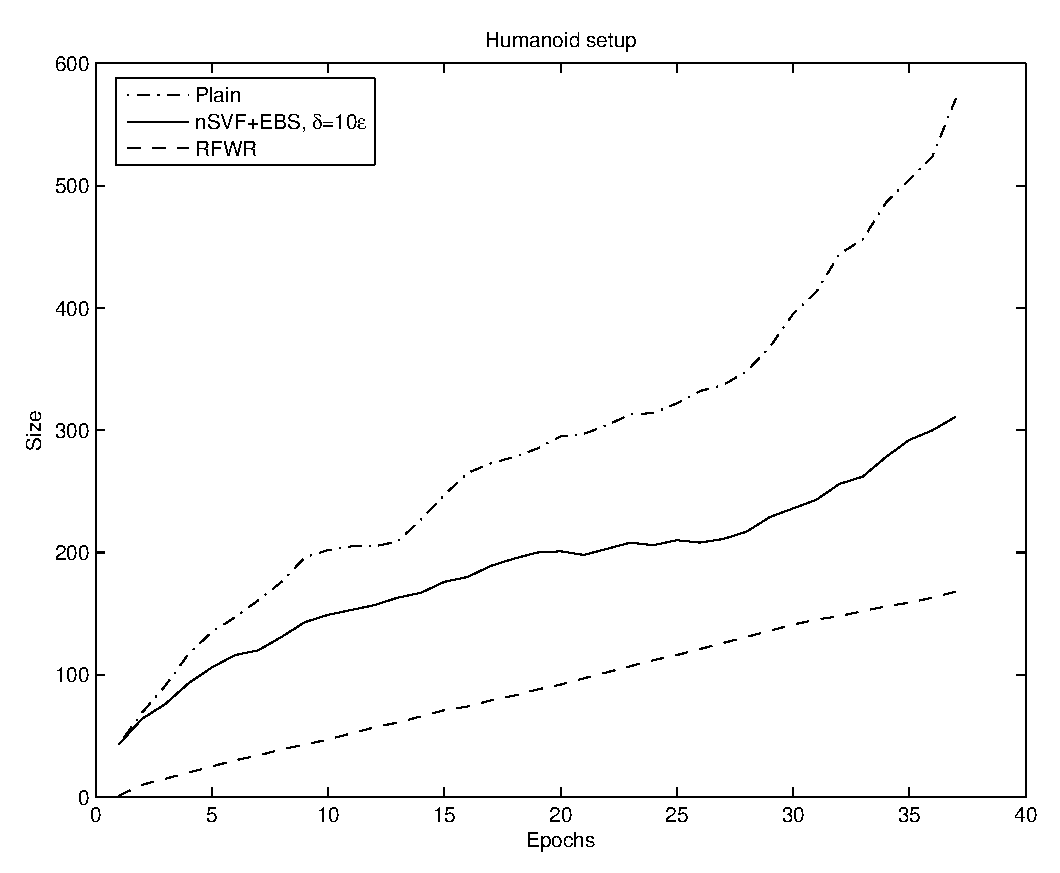
\includegraphics[width=0.45\textwidth]{fig2b} \\[5mm]
       \multicolumn{2}{c}{
         \begin{tabular}{|l|r|r|}
           \hline
           Machine & Size & MSE \\
           \hline\hline
           Plain                    &$100\%$   & $0.0473$ \\
           EBS, $\delta=10\epsilon$ & $85.3\%$ & $0.0477$ \\
           EBS, $\delta=50\epsilon$ & $29.3\%$ & $0.0788$ \\
           \bf nSVF+EBS, $\delta=10\epsilon$ &  $54.7\%$ & $0.0557$ \\
           \hline
         \end{tabular}
       }
    \end{tabular}
  \end{center}
  \caption{\label{fig:hum} Experimental results for the arm/hand/eye
    humanoid mapping (see Subsection \ref{subs:kinmod}). \emph{Above
    left:} percentage of the plain machine size, as a function of the
    epochs. Comparison among EBS with $\delta=10\epsilon$, EBS with
    $\delta=50\epsilon$ and nSVF+EBS with
    $\delta=10\epsilon$. \emph{Above right:} The strategy with the
    best trade-off as resulting from the Left panel, i.e., nSVF+EBS
    with $\delta=10\epsilon$, compared with the plain SVM and Schaal's
    RFWR. \emph{Below:} numerical data: for each plotted machine,
    final size as a percentage of the plain SVM and MSE of the
    regressions obtained. The strategy with the best tradeoff appears
    in boldface.}
\end{figure*}

The Figures and table indicate that the results are not very different
from those outlined in the previous Subsection. The size versus
accuracy tradeoff is confirmed. In this case the best-tradeoff
strategy appears to be nSVF+EBS with $\delta=10\epsilon$, which keeps
the machine slightly bigger than half of the plain SVM, and still
about double the RFWR. In this case, however, the MSE achieved by RFWR
is very large (slightly less than $0.3$) but it is not comparable with
ours, since the RFWR strategy needs many more epochs to achieve a good
training, and this experiment has probably too few samples.

\subsection{Discussion}

The message we gather is the following: some simple ideas to filter
out the samples as one explores the input space of a learning system
can greatly improve the time and space requirements of the machines
involved. In particular, from the experimental tests:

\begin{itemize}

  \item The nSVF strategy, that is, removing whatever is not a support
    vector, is good --- it appears in both best-trade-off
    strategies. This agrees with the already cited paper
    \cite{syed99incremental} (see Section \ref{sec:opt}).

  \item All in all, the loss in performance is not bad, also if one
    wants to have very small machines. Consider the numerical tables
    in this Section, and compare the MSE of the smallest machines
    with that of the plain SVM: it is about $2.7$ times higher in the
    teleoperation problem, and $1.67$ times in the humanoid
    problem. But the machine sizes are, in turn, less than \emph{one
    tenth} and less than $30\%$ than of plain SVMs.

  \item As far as timings are concerned, at the end of the considered
    epochs, the training time is about $3.6\%$ and $18\%$ of the plain
    SVM, in turn, for the two problems considered. This is in rough
    agreement with the theory, according to which the training time is
    cubic in the number of support vectors of a SVM
    \cite{KeerthiCDC06}.

\end{itemize}

We believe that especially the last point paves the way to the use of
SVMs in on-line robotic control applications. Notice, as a final
remark, that the strategies presented are not problem-dependent,
meaning that they can be in principle applied to any regression
problem whatsoever. This does not mean, of course, that they will be
this effective on any other problem.

\section{Conclusions}
\label{sec:concl}

In this paper we have presented three optimisation strategies which
effectively reduce the size (and hence, the training time) of Support
Vector Machines applied to two problems of robotic control. The
optimisations are problem-independent, meaning that they can in
principle be applied to any other SVM-based regression problem (this
does not mean that they will be effective on all problems, of
course). The resulting, smaller machines retain most of the accuracy
of the non-reduced ones. As far as we know, this is one of the first
attempts at using SVMs for robotic control.

Future work will mainly develop along these lines: $(i)$ building
online versions of these machines and actually using them on the
described setups, $(ii)$ theoretically characterising the advantages
that the presented optimisations give. A strand we are already
pursuing is that of linking the total number of support vectors a
machine should consider to the Vapnik-Chervonenkis dimension of the
kernel used, \emph{without losing accuracy}. Preliminary results are
encouraging.

\section*{Acknowledgements}

The authors would like to thank Giorgio Metta for invaluable
discussions on the subject. The work here presented is partially
supported by the project Neurobotics (IST-FP6-001917). For more
informations, see \url{http://www.neurobotics.info}.

\bibliographystyle{IEEEtran}
\bibliography{paper}

\end{document}
